\documentclass{sigkdd}
\usepackage{blindtext}

\usepackage{color}
\usepackage{tikz}
\usetikzlibrary{arrows}


\title{Message Passing and Expectation Propagation}
\subtitle{Efficient Inference in large scale machine learning}
\numberofauthors{1}
\author{
\alignauthor Christoph Dehner \\
\affaddr{Department of Informatics}\\
\affaddr{Technische Universit\"at M\"unchen}\\
\email{dehner@in.tum.de}
}



\begin{document}
\maketitle

% Abstract
\begin{abstract}
\blindtext
\end{abstract}

\section{Introduction}
Probabilistic graphical models like Markov Random Fields or Bayesian Networks provide clear and illustrative ways to describe probabilistic processes. In such models, nodes represent random variables and edges their conditional dependencies. The joint distribution of all involved variables can be expressed as a product of factors, which are observed or given specific values during modelling. As an example, a Bayesian network with three variables is given in figure \ref{fig:BN}. It defines the values of $x_1$ and $x_3$ to be conditionally independent given $x_2$.
\begin{figure}[h]
	\centering
	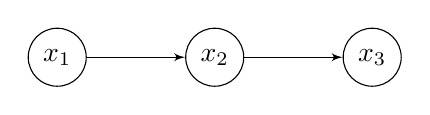
\begin{tikzpicture}
	
	\tikzset{vertex/.style = {shape=circle,draw,minimum size=1.5em}}
	\tikzset{edge/.style = {->,> = latex'}}
	
	\node[vertex] (x1) at  (0,0) {$x_1$};
	\node[vertex] (x2) at  (2,0) {$x_2$};
	\node[vertex] (x3) at  (4,0) {$x_3$};
	
	\draw[edge] (x1) to (x2);
	\draw[edge] (x2) to (x3);
	\end{tikzpicture}
	\caption{Bayesian network with three variables. $x_1$ and $x_3$ are conditionally independent given $x_2$.}\label{fig:BN}
\end{figure}

Typical tasks in such a scenario are to do Bayesian inference to extract marginal distribution of specific variables or find maximum apriori estimates. However, with an increasing number of variables these task can become computationally very expensive. 

The naive approach for marginalisation is to sum out all but one variable from the joint distribution $p(X)$. This is formally shown in equation \ref{eq:marginalisation_naive}, where $X \setminus x_i$ describes the set of all random variables expect $x_i$.
This strategy requires exponentially in the number of variables many evaluations of the joint distribution and is thus not applicable to bigger networks.
\begin{equation}\label{eq:marginalisation_naive}
p(x_i)= \sum_{X \setminus x_i} p(\mathbf{x})
\end{equation}
Therefore, this paper explains more efficient algorithms to do large scale Bayesian inference in graphical models. The next chapter $todo$ deals with exact inference and presents two message passing algorithms to calculate marginals and maximum apriori estimates for graphical models. Subsequently, in chapter $todo$ expectation propagation as a method of approximate inference is explained.

\section{Exact inference}
The intuition of the algorithms presented in this section is to exploit independence properties of the random variables. Graphical models define the joint probability to be expressed as a product of factors, considering the conditional independences expressed by the graph. For Bayesian networks those factors correspond to conditional distributions, in Markov Random Fields to clique potentials. Assuming appropriately normalized factors, the joint distribution can be written as a product according to equation \ref{eq:product_of_factors}. The index $s$ iterates here over all factors of the graph; $X_s$ defines the subset of variables, the factor $s$ depends on.
\begin{equation}\label{eq:product_of_factors}
p(X)= \prod_{s} f_s(X_s)
\end{equation}
Expressing the joint distribution as the product defined by the graph allows to exchange summations and multiplications during marginalization. By this way, marginalization can often be done a lot more efficient. Equation \ref{eq:marginalization_smart} demonstrates this transformation with the Bayesian network from figure \ref{fig:BN}, whose joint distribution $p(X)$ is defined as $p(X) =  p(x_1) p(x_2|x_1) p(x_3|x_1)$.
\begin{equation}\label{eq:marginalization_smart}
\begin{split}
p(x_2) &= \sum_{x_1} \sum_{x_3} p(x_1) p(x_2|x_1) p(x_3|x_2) \\ &= \sum_{x_1} \Big[  p(x_1) p(x_2|x_1) \sum_{x_3} \Big[ p(x_3|x_2)\Big] \Big] \\ &= \underbrace{\Big[ \sum_{x_1}  p(x_1) p(x_2|x_1)\Big]}_{\mu_{x_1 \rightarrow x_2}}\cdot \underbrace{\Big[ \sum_{x_3}  p(x_3|x_2)\Big]}_{\mu_{x_3 \rightarrow x_2}}
\end{split}
\end{equation}
Here, the sum of products from the naive approach for marginalization is transformed to a product of sums, reducing the exponential computational complexity in the number of random variables to linear effort.

The brackets in the last line of equation \ref{eq:marginalization_smart} reveal a powerful interpretation of the marginalizing. The marginal distribution $p(x_2)$ consists of two messages $\mu_{x_1 \rightarrow x_2}$ and $\mu_{x_3 \rightarrow x_2}$ from its neighboring cells $x_1$ and $x_3$. For a longer chain of random variables these messages would again be comprised by messages from their neighboring cell. Applied to a chain of arbitrary length, this method gives a recursive pattern in which messages for the marginalization are sent to the marginalized variable node from both ends of the chain.  

This message passing idea is the foundation for the two inference algorithms presented in this chapter subsequently. Before that the next section introduces factor graphs, the structure these algorithms operate on.

\subsection{Factor graphs}
Factor graphs make the factorisation of a joint probability distribution explicit. The can be generated from Bayesian networks as well as from Markov random fields and thus allow to define inference algorithms independent of how the underlying probabilistic graphical model was introduced.

Additional to the variable nodes, a factor graph also consists of factor nodes representing the factors of the decomposed joint probability distribution as in equation  \ref{eq:product_of_factors}. Edges connect the factor nodes to all variables they depend on. By this way they a bipartite graph with variable nodes (usually visualised by circles) on the one side and and factors (depicted as rectangles) on the other side.

Depending on the exact factorisation, a distribution defined by a Bayesian network or Markov random field can be represented by different factor graphs. Figure $todo$ depicts a factor graph of the Bayesian network from figure \ref{fig:BN}, in which all conditional distribution are represented by separate factors.

The inference algorithms on factor graphs of the following sections are valid for trees. Such factor graphs with exactly one path between any pair of nodes can be generated from undirected trees in the case of a Markov random field model as well as from from directed trees and polytrees, if the factor graph is derived from a Bayesian network. More detailed description how to derive factor graph from probabilistic graph models can be found in \textcolor{red}{todo: add reference}.



\subsection{Marginalization}
The sum-product algorithm presented in this section generalises the idea of exchanging summation and multiplication during marginalisation. It consists of local messages passed between factor and variable nodes in a factor graph.

As a starting point let us consider the calculation of the marginal distribution $p(x_i)$ in the factor graph of figure \ref{fig:message1}. Furthermore we define $F_s(s, X_s)$ for all neighbours $s$ of $x_i$ as the product of all factors in the respective sub-tree of the neighbour. This is visualised by blue circles in figure \ref{fig:message1}.
\begin{figure}[h]
	\centering
	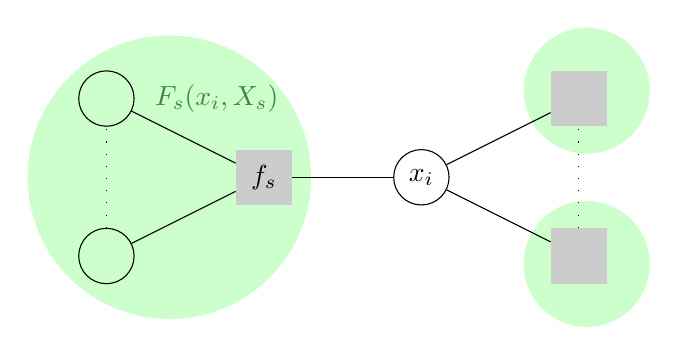
\begin{tikzpicture}
	
	\definecolor{darkgreen}{RGB}{59,136,59}
	
	\tikzstyle{edge} = [draw,-]
    \fill[green!20]   (0:-1.2) circle (1.8);
    \node[darkgreen] (text) at (-0.6,1) {$F_s(x_i,X_s)$};
    
    \fill[green!20]   (4.1,-1.1) circle (0.8);
    \fill[green!20]   (4.1,1.1) circle (0.8);

	\tikzset{vertex/.style = {shape=circle,draw,minimum size=2em}}
	\node[vertex] (xi) at  (2,0) {$x_i$};
	\node[vertex] (xl1) at  (-2,-1) {};
	\node[vertex] (xl2) at  (-2,1) {};
	
	\tikzset{vertex/.style = {shape = rectangle,fill = gray!40,minimum size=2em}}
	\node[vertex] (fs) at  (0,0) {$f_s$};
	\node[vertex] (xr1) at  (4,-1) {};
	\node[vertex] (xr2) at  (4,1) {};
	
	\draw[edge] (fs) to (xi);
	\draw[edge] (xi) to (xr1);
	\draw[edge] (xi) to (xr2);
	\draw[edge] (fs) to (xl1);
	\draw[edge] (fs) to (xl2);
	\draw[edge, loosely dotted] (xr1) to (xr2);
	\draw[edge, loosely dotted] (xl1) to (xl2);
	\end{tikzpicture}
	\caption{Exemplary factor graph to deduce the messages of the sum-product algorithm.}\label{fig:message1}
\end{figure}

Analogous to the general factorisation defined by the graphical model from equation \ref{eq:product_of_factors} the joint probability $p(\mathbf{x})$ can then be expressed as a product of those neighbour-factor of $x_i$:
\begin{equation}\label{eq:product_of_neighbours}
p(X)= \prod_{s \in ne(x_i)} F_s(x_i, X_s)
\end{equation}
Inserting this representation of the joint distribution in the naive marginalisation formula from equation \ref{eq:marginalisation_naive} allows to exchange sum and product. By this way the marginal distribution of $x_i$ is expressed as the product of messages $\mu_{f_s \rightarrow x_i}$ from all its neighbours in the factor graph:
\begin{equation}\label{eq:message1}
\begin{split}
p(x_i) &= \sum_{X \setminus x_i} \Big[ \prod_{s \in ne(x_i)} F_s(x_i, X_s) \Big] \\ &= \prod_{s \in ne(x_i)} \Big[ \sum_{X_s} F_s(x_i, X_s)\Big] =: \prod_{s \in ne(x_i)} \mu_{f_s \rightarrow x_i}
\end{split}
\end{equation}

The factors $F_s(x,X_s)$ represent subtrees in the factor graphs and can thus be factorized again: 
\begin{equation}\label{eq:product_of_neighbours}
F_s(x_i,X_s) = f_s(x_i, X_s) G_1(x_1, X_{s_1})\dots G_1(x_M, X_{s_M}).
\end{equation}
The factors $G_1(x_1, X_{s_1})\dots G_1(x_M, X_{s_M})$ represent here the subgraphs of all neighbours of $f_s$ except from $x_i$ and are illustrated by red circles in figure \ref{fig:message2}.

\begin{figure}[h]
	\centering
	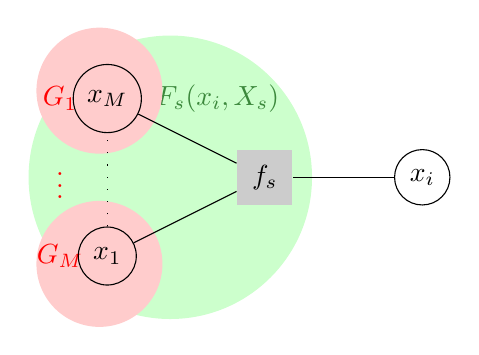
\begin{tikzpicture}
	
	\definecolor{darkgreen}{RGB}{59,136,59}
	
	\tikzstyle{edge} = [draw,-]
    \fill[green!20]   (0:-1.2) circle (1.8);
    \node[darkgreen] (text) at (-0.6,1) {$F_s(x_i,X_s)$};
    
    \fill[red!20]   (-2.1,-1.1) circle (0.8);
    \fill[red!20]   (-2.1,1.1) circle (0.8);
    \node[red] (text) at (-2.6,1) {$G_1$};
    \node[red] (text) at (-2.6,0) {$\vdots$};
    \node[red] (text) at (-2.6,-1) {$G_M$};


	\tikzset{vertex/.style = {shape=circle,draw,minimum size=2em}}
	\node[vertex] (xi) at  (2,0) {$x_i$};
	\node[vertex] (xl1) at  (-2,-1) {$x_1$};
	\node[vertex] (xl2) at  (-2,1) {$x_M$};
	
	\tikzset{vertex/.style = {shape = rectangle,fill = gray!40,minimum size=2em}}
	\node[vertex] (fs) at  (0,0) {$f_s$};
	
	\draw[edge] (fs) to (xi);
	\draw[edge] (fs) to (xl1);
	\draw[edge] (fs) to (xl2);
	\draw[edge, loosely dotted] (xl1) to (xl2);
	\end{tikzpicture}
	\caption{Exemplary factor graph to deduce the messages of the sum-product algorithm.}\label{fig:message2}
\end{figure}

With that, the messages defined in equation \ref{eq:product_of_neighbours} can be further evaluated to
\begin{equation}\label{eq:message2}
\begin{split}
\mu_{f_s \rightarrow x_i}(x_i) &= \sum_{X_s \setminus x_i} f_s(x_i, X_s) \prod_{m \in ne(f_s) \setminus x_i} \Big[ \sum_{{X_s}_m} G_m(x_m, {X_s}_m)  \Big] \\ &= \sum_{\mathbf{x_s} \setminus x_i} f_s(x_i, X_s) \prod_{m \in ne(f_s) \setminus x_i} \mu_{x_m \rightarrow f_s}(x_m).
\end{split}
\end{equation}
We have now defined  messages from factor to variable nodes. $\mu_{x_m \rightarrow f_s}(x_m) :=\sum_{{X_s}_m} G_m(x_m, {X_s}_m)$. Going one step further yields an expression for messages from variables to factors as well. Analogously to before, $G_m(x_m, {X_s}_m)$ can be factorised again to 
\begin{equation}\label{eq:product_of_neighbours2}
G_m(x_m,{X_s}_m) = \prod_{l \in ne(x_m) \setminus f_s} F_l(x_m, {{X_s}_m}_l),
\end{equation}
as visualised in figure \ref{fig:message3}.

\begin{figure}[h]
	\centering
	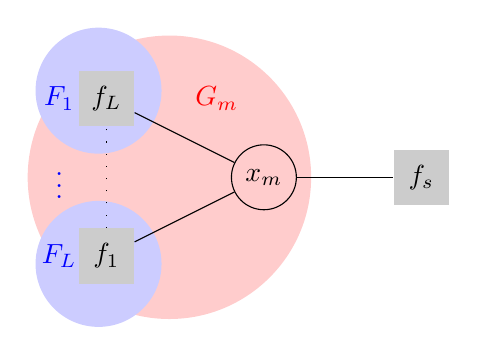
\begin{tikzpicture}
	
	\definecolor{darkgreen}{RGB}{59,136,59}
	
	\tikzstyle{edge} = [draw,-]
    \fill[red!20]   (0:-1.2) circle (1.8);
    \node[red] (text) at (-0.6,1) {$G_m$};
    
    \fill[blue!20]   (-2.1,-1.1) circle (0.8);
    \fill[blue!20]   (-2.1,1.1) circle (0.8);
    \node[blue] (text) at (-2.6,1) {$F_1$};
    \node[blue] (text) at (-2.6,0) {$\vdots$};
    \node[blue] (text) at (-2.6,-1) {$F_L$};

	\tikzset{vertex/.style = {shape = rectangle,fill = gray!40,minimum size=2em}}
	\node[vertex] (xi) at  (2,0) {$f_s$};
	\node[vertex] (xl1) at  (-2,-1) {$f_1$};
	\node[vertex] (xl2) at  (-2,1) {$f_L$};
	
	\tikzset{vertex/.style = {shape=circle,draw,minimum size=2em}}
	\node[vertex] (fs) at  (0,0) {$x_m$};
	
	\draw[edge] (fs) to (xi);
	\draw[edge] (fs) to (xl1);
	\draw[edge] (fs) to (xl2);
	\draw[edge, loosely dotted] (xl1) to (xl2);
	\end{tikzpicture}
	\caption{Exemplary factor graph to deduce the messages of the sum-product algorithm.}\label{fig:message3}
\end{figure}

Inserting this factorisation into the definition of $\mu_{x_m \rightarrow f_s}(x_m)$ and exchanging summation and multiplication reveals an explicite formulat for this messages:
\begin{equation}\label{eq:product_of_neighbours3}
    \begin{split}
        \mu_{x_m \rightarrow f_s}(x_m) &=\sum_{{X_s}_m} \Big[ \prod_{l \in ne(x_m) \setminus f_s} F_l(x_m, {{X_s}_m}_l) \Big] \\ &= \prod_{l \in ne(x_m) \setminus f_s} \Big[\sum_{{{X_s}_m}_l} F_l(x_m, {{X_s}_m}_l) \Big] \\ &= \prod_{l \in ne(x_m) \setminus f_s} \mu_{f_l \rightarrow x_m}(x_m)
    \end{split}
\end{equation}

We have now induced how a marginal distribution $p(x_i)$ can be expressed by local messages passed between factors and variables through the factor graph. For leave nodes those messages can be stated explicitely.
For a variable node as leave of the factor graph equation \ref{eq:product_of_neighbours3} shows that the message, the node sends to its only neighbor, is given by
\begin{equation}\label{eq:product_of_neighbours3}
\mu_{x \rightarrow f}(x) = 1.
\end{equation}
Similarly, from equation \ref{eq:product_of_neighbours2} then concludes the initial value
\begin{equation}\label{eq:product_of_neighbours3}
\mu_{f \rightarrow x}(x) = f(x)
\end{equation}
for a message from a leave factor node to its neighbouring variable node.

Having explicit start values for messages from the leaves, messages can propagated through the factor graphs to an arbitrarly chosen root node. This root node has then recieved messages from all its neighbours and can thus calculate its marginal distribution according to \ref{eq:message1}. Analogously, passing all messages back from the root to all leave nodes enables to calculate the marginals of all variables in the factor graph. For this calculation two time the number of edges in the factor graph many messages have to be computed, which is linear in the number of variables of the model.  
\textcolor{red}{todo: marginal of a factor formula}


\subsection{Maximum Apriori Estimate}
Problemformulierung
max-sum-algorithms

\subsection{Inference in general graphs}
loopy belief propagation

\section{Approximate inference}
Known as expectation propagation, similar to variational inference
Minimize KL-divergence using moment matching.
Interesting properties different from standard VI
\subsection{Methodology}
\subsection{Expectation propagation in graphical models}

\section{Summary and outlook}


% Subsections
\subsection{Subsection}
blabla with 2 sources \cite{murphy2012machine, bishop2006prml}.

% Example figure
\begin{figure}[h]
	\begin{center}
		\includegraphics[scale=0.2]{figure1.png}
		\caption{Tree}\label{fig:tree}
	\end{center}
\end{figure}

% Example table
\begin{table}[h]
	\begin{center}
		\caption{Example table}\label{tab:example}
		\begin{tabular}{c|c}
			Column 1 & Column 2\\
			\hline
			0 & 1\\
		\end{tabular}
	\end{center}
\end{table}

% Bibliography
\bibliographystyle{abbrv}
% Add references using the command below
\bibliography{references}

\end{document}